\documentclass[../main.tex]{subfiles}

\begin{document}

\chapter{Splines and Piecewise Interpolation}\label{chap:chap18}

\begin{center}
    \Large{\textbf{CHAPTER OBJECTIVES}}
\end{center}
The primary objective of this chapter is to introduce you to splines. Specific objectives
and topics covered are:

\begin{itemize}
    \item Understanding that splines minimize oscillations by fitting lower-order
    polynomials to data in a piecewise fashion.
    \item Knowing how to develop code to perform a table lookup.
    \item Recognizing why cubic polynomials are preferable to quadratic and higher-order
    splines.
    \item Understanding the conditions that underlie a cubic spline fit.
    \item Understanding the differences between natural, clamped, and not-a-knot end
    conditions.
    \item Knowing how to fit a spline to data with MATLAB's built-in functions
    \item Understanding how multidimensional interpolation is implemented with MATLAB.
\end{itemize}
\vspace{2cm}
\section{INTRODUCTION TO SPLINES}
In Chap. 17 (n - 1)th-order polynomials were used to interpolate between n data points.
For example, for eight points, we can derive a perfect seventh-order polynomial. This
curve would capture all the meanderings (at least up to and including seventh derivatives)
suggested by the points. However, there are cases where these functions can lead to erroneous results because of round-off error and oscillations. An alternative approach is to
apply lower-order polynomials in a piecewise fashion to subsets of data points. Such connecting polynomials are called spline functions.
For example, third-order curves employed to connect each pair of data points are
called cubic splines. These functions can be constructed so that the connections between
\begin{figure}[H]
    \centering
    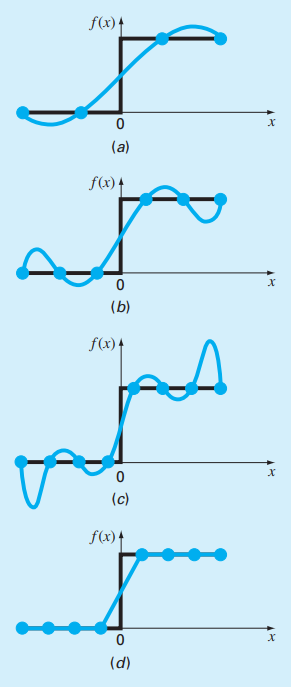
\includegraphics[scale=0.6]{fig_18_1}
   \caption{\textsf{A visual representation of a situation where splines are superior to higher-order interpolating
   polynomials. The function to be fit undergoes an abrupt increase at x = 0. Parts (a) through (c)
   indicate that the abrupt change induces oscillations in interpolating polynomials. In contrast,
   because it is limited to straight-line connections, a linear spline (d) provides a much more
   acceptable approximation.}}\label{fig:fig_18_1}
\end{figure}
adjacent cubic equations are visually smooth. On the surface, it would seem that the thirdorder approximation of the splines would be inferior to the seventh-order expression. You
might wonder why a spline would ever be preferable.
Figure 18.1 illustrates a situation where a spline performs better than a higher-order
polynomial. This is the case where a function is generally smooth but undergoes an abrupt
change somewhere along the region of interest. The step increase depicted in Fig. 18.1 is
an extreme example of such a change and serves to illustrate the point.
Figure 18.1a through c illustrates how higher-order polynomials tend to swing through
wild oscillations in the vicinity of an abrupt change. In contrast, the spline also connects
the points, but because it is limited to lower-order changes, the oscillations are kept to a
\begin{figure}[H]
    \centering
    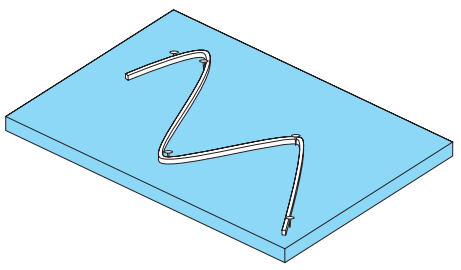
\includegraphics[scale=0.6]{fig_18_2}
   \caption{\textsf{The drafting technique of using a spline to draw smooth curves through a series of points. Notice
   how, at the end points, the spline straightens out. This is called a “natural” spline.}}\label{fig:fig_18_2}
\end{figure}

minimum. As such, the spline usually provides a superior approximation of the behavior of
functions that have local, abrupt changes.
The concept of the spline originated from the drafting technique of using a thin, flexible strip (called a spline) to draw smooth curves through a set of points. The process is depicted in Fig. 18.2 for a series of five pins (data points). In this technique, the drafter places
paper over a wooden board and hammers nails or pins into the paper (and board) at the location of the data points. A smooth cubic curve results from interweaving the strip between
the pins. Hence, the name “cubic spline” has been adopted for polynomials of this type.
In this chapter, simple linear functions will first be used to introduce some basic concepts and issues associated with spline interpolation. Then we derive an algorithm for fitting
quadratic splines to data. This is followed by material on the cubic spline, which is the most
common and useful version in engineering and science. Finally, we describe MATLAB's
capabilities for piecewise interpolation including its ability to generate splines.
\section{LINEAR SPLINES}
The notation used for splines is displayed in Fig. 18.3. For n data points (i = 1, 2,..., n),
there are n - 1 intervals. Each interval i has its own spline function, $s\textsubscript{i}$(x). For linear
splines, each function is merely the straight line connecting the two points at each end of
the interval, which is formulated as
\begin{equation}
    \tag{18.1}
    s_{i}(x)=a_{i}+b_{i}\left(x-x_{i}\right)
\end{equation}
where $a\textsubscript{i}$ is the intercept, which is defined as
\begin{equation}
    \tag{18.2}
    a_{i}=f_{i}
\end{equation}
and $b\textsubscript{i}$ is the slope of the straight line connecting the points:
\begin{equation}
    b_{i}=\frac{f_{i+1}-f_{i}}{x_{i+1}-x_{i}}
    \tag{18.3}
    \end{equation}
    \begin{figure}[H]
        \centering
        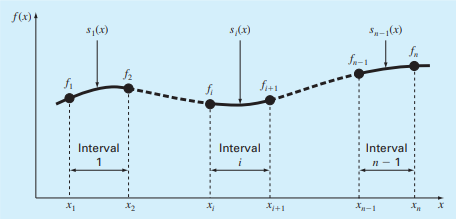
\includegraphics[scale=0.8]{fig_18_3}
       \caption{\textsf{Notation used to derive splines. Notice that there are n - 1 intervals and n data points.}}\label{fig:fig_18_3}
    \end{figure}
    where $f\textsubscript{i}$ is shorthand for f ($x\textsubscript{i}$). Substituting Eqs. (18.1) and (18.2) into Eq. (18.3) gives
    \begin{equation}
        s_{i}(x)=f_{i}+\frac{f_{i+1}-f_{i}}{x_{i+1}-x_{i}}\left(x-x_{i}\right)
        \tag{18.4}
    \end{equation}
    These equations can be used to evaluate the function at any point between x1 and xn
by first locating the interval within which the point lies. Then the appropriate equation is
used to determine the function value within the interval. Inspection of Eq. (18.4) indicates
that the linear spline amounts to using Newton's first-order polynomial [Eq. (17.5)] to
interpolate within each interval.

\begin{exmp} \textbf{First-Order Splines}
    \noindent\textit{Problem Statement.} Fit the data in Table 18.1 with first-order splines. Evaluate the
    function at x = 5.
    \begin{equation}
        \begin{aligned}
        &\text { TABLE 18.1 Data to be fit with spline functions. }\\
        &\begin{array}{ccc}
        \hline \boldsymbol{i} & \boldsymbol{x}_{\boldsymbol{i}} & \boldsymbol{f}_{\boldsymbol{i}} \\
        \hline 1 & 3.0 & 2.5 \\
        2 & 4.5 & 1.0 \\
        3 & 7.0 & 2.5 \\
        4 & 9.0 & 0.5 \\
        \hline
        \nonumber
        \end{array}
        \end{aligned}
        \end{equation}
        \noindent \textbf{Solution.} The data can be substituted into Eq. (18.4) to generate the linear spline
        functions. For example, for the second interval from x = 4.5 to x = 7, the function is
        \begin{equation}
            s_{2}(x)=1.0+\frac{2.5-1.0}{7.0-4.5}(x-4.5) \nonumber
            \end{equation}

            \begin{figure}[H]
                \centering
                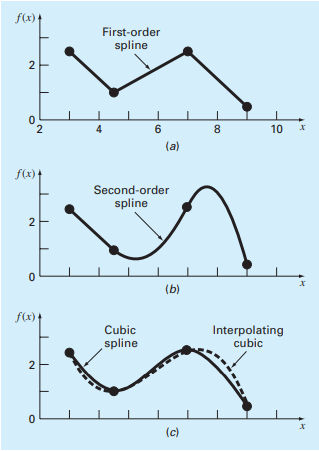
\includegraphics[scale=0.6]{fig_18_4}
               \caption{\textsf{Spline fits of a set of four points. (a) Linear spline, (b) quadratic spline, and (c) cubic spline, with
               a cubic interpolating polynomial also plotted.}}\label{fig:fig_18_4}
            \end{figure}
            The equations for the other intervals can be computed, and the resulting first-order splines
are plotted in Fig. 18.4a. The value at x = 5 is 1.3.
\begin{equation}
    s_{2}(x)=1.0+\frac{2.5-1.0}{7.0-4.5}(5-4.5)=1.3 \nonumber
    \end{equation}

    \end{exmp} 

    Visual inspection of Fig. 18.4a indicates that the primary disadvantage of first-order
splines is that they are not smooth. In essence, at the data points where two splines meet
(called a knot), the slope changes abruptly. In formal terms, the first derivative of the function is discontinuous at these points. This deficiency is overcome by using higher-order
polynomial splines that ensure smoothness at the knots by equating derivatives at these
points, as will be discussed subsequently. Before doing that, the following section provides
an application where linear splines are useful.
\subsection{Table Lookup}

A table lookup is a common task that is frequently encountered in engineering and science
computer applications. It is useful for performing repeated interpolations from a table of
independent and dependent variables. For example, suppose that you would like to set up
an M-file that would use linear interpolation to determine air density at a particular temperature based on the data from Table 17.1. One way to do this would be to pass the M-file
the temperature at which you want the interpolation to be performed along with the two adjoining values. A more general approach would be to pass in vectors containing all the data
and have the M-file determine the bracket. This is called a table lookup.
Thus, the M-file would perform two tasks. First, it would search the independent variable vector to find the interval containing the unknown. Then it would perform the linear
interpolation using one of the techniques described in this chapter or in Chap. 17.
For ordered data, there are two simple ways to find the interval. The first is called a
sequential search. As the name implies, this method involves comparing the desired value
with each element of the vector in sequence until the interval is located. For data in ascending order, this can be done by testing whether the unknown is less than the value being
assessed. If so, we know that the unknown falls between this value and the previous one
that we examined. If not, we move to the next value and repeat the comparison. Here is a
simple M-file that accomplishes this objective:
\begin{lstlisting}[numbers=none]
    function yi = TableLook(x, y, xx)
    n = length(x);
    if xx < x(1) | xx > x(n)
    error('Interpolation outside range')
    end
    % sequential search
    i = 1;
    while(1)
    if xx <= x(i + 1), break, end
    i = i + 1;
    end
    % linear interpolation
    yi = y(i) + (y(i+1)-y(i))/(x(i+1)-x(i))*(xx-x(i));
\end{lstlisting}

The table’s independent variables are stored in ascending order in the array x and the
dependent variables stored in the array y. Before searching, an error trap is included to ensure that the desired value xx falls within the range of the x’s. A while . . . break loop
compares the value at which the interpolation is desired, xx, to determine whether it is less
than the value at the top of the interval, x(i+1). For cases where xx is in the second interval or higher, this will not test true at first. In this case the counter i is incremented by one
so that on the next iteration, xx is compared with the value at the top of the second interval. The loop is repeated until the xx is less than or equal to the interval’s upper bound, in
which case the loop is exited. At this point, the interpolation can be performed simply as
shown.
For situations for which there are lots of data, the sequential sort is inefficient because
it must search through all the preceding points to find values. In these cases, a simple
alternative is the binary search. Here is an M-file that performs a binary search followed
434 SPLINES AND PIECEWISE INTERPOLATION
by linear interpolation:
\begin{lstlisting}[numbers=none]
    function yi = TableLookBin(x, y, xx)
    n = length(x);
    if xx < x(1) | xx > x(n)
    error('Interpolation outside range')
    end
    % binary search
    iL = 1; iU = n;
    while (1)
    if iU - iL <= 1, break, end
    iM = fix((iL + iU) / 2);
    if x(iM) < xx
    iL = iM;
    else
    iU = iM;
    end
    end
    % linear interpolation
    yi = y(iL) + (y(iL+1)-y(iL))/(x(iL+1)-x(iL))*(xx - x(iL));
\end{lstlisting}

The approach is akin to the bisection method for root location. Just as in bisection, the
index at the midpoint iM is computed as the average of the first or “lower” index iL = 1
and the last or “upper” index iU = n. The unknown xx is then compared with the value of
x at the midpoint x(iM) to assess whether it is in the lower half of the array or in the upper
half. Depending on where it lies, either the lower or upper index is redefined as being the
middle index. The process is repeated until the difference between the upper and the lower
index is less than or equal to zero. At this point, the lower index lies at the lower bound of
the interval containing xx, the loop terminates, and the linear interpolation is performed.
Here is a MATLAB session illustrating how the binary search function can be applied
to calculate the air density at 350 °C based on the data from Table 17.1. The sequential
search would be similar.
\begin{lstlisting}[numbers=none]
    >> T = [-40 0 20 50 100 150 200 250 300 400 500];
    >> density = [1.52 1.29 1.2 1.09 .946 .935 .746 .675 .616...
    .525 .457];
    >> TableLookBin(T,density,350)
    ans =
    0.5705
\end{lstlisting}

This result can be verified by the hand calculation:
\begin{equation}
    f(350)=0.616+\frac{0.525-0.616}{400-300}(350-300)=0.5705 \nonumber
    \end{equation}

\section{QUADRATIC SPLINES}

To ensure that the nth derivatives are continuous at the knots, a spline of at least n + 1
order must be used. Third-order polynomials or cubic splines that ensure continuous first
and second derivatives are most frequently used in practice. Although third and higher
derivatives can be discontinuous when using cubic splines, they usually cannot be detected
visually and consequently are ignored.
Because the derivation of cubic splines is somewhat involved, we have decided to first
illustrate the concept of spline interpolation using second-order polynomials. These “quadratic splines” have continuous first derivatives at the knots. Although quadratic splines are
not of practical importance, they serve nicely to demonstrate the general approach for developing higher-order splines.
The objective in quadratic splines is to derive a second-order polynomial for each interval between data points. The polynomial for each interval can be represented generally as

\begin{equation}
    \tag{18.5}
    s_{i}(x)=a_{i}+b_{i}\left(x-x_{i}\right)+c_{i}\left(x-x_{i}\right)^{2}
\end{equation}

where the notation is as in Fig. 18.3. For n data points (i = 1, 2,..., n), there are n - 1
intervals and, consequently, 3(n - 1) unknown constants (the a's, b's, and c's) to evaluate.
Therefore, 3(n - 1) equations or conditions are required to evaluate the unknowns. These
can be developed as follows:
\begin{enumerate}
    \item The function must pass through all the points. This is called a continuity condition. It
    can be expressed mathematically as
\begin{equation}
    f_{i}+b_{i}\left(x_{i+1}-x_{i}\right)+c_{i}\left(x_{i+1}-x_{i}\right)^{2}=f_{i+1}+b_{i+1}\left(x_{i+1}-x_{i+1}\right)+c_{i+1}\left(x_{i+1}-x_{i+1}\right)^{2}
    \nonumber
\end{equation}
which simplifies to

\begin{equation}
    \tag{18.6}
    a_{i}=f_{i}
\end{equation}
Therefore, the constant in each quadratic must be equal to the value of the dependent
variable at the beginning of the interval. This result can be incorporated into Eq. (18.5):
\begin{equation}
    s_{i}(x)=f_{i}+b_{i}\left(x-x_{i}\right)+c_{i}\left(x-x_{i}\right)^{2} \nonumber
    \end{equation}
    Note that because we have determined one of the coefficients, the number of conditions to be evaluated has now been reduced to 2(n - 1).

    \item The function values of adjacent polynomials must be equal at the knots. This condition
    can be written for knot i + 1 as
    \begin{equation}
        \tag{18.7}
        f_{i}+b_{i}\left(x_{i+1}-x_{i}\right)+c_{i}\left(x_{i+1}-x_{i}\right)^{2}=f_{i+1}+b_{i+1}\left(x_{i+1}-x_{i+1}\right)+c_{i+1}\left(x_{i+1}-x_{i+1}\right)^{2}
        \end{equation}
        This equation can be simplified mathematically by defining the width of the ith interval as
        \begin{equation}
            h_{i}=x_{i+1}-x_{i} \nonumber
            \end{equation}
Thus, Eq. (18.7) simplifies to
\begin{equation}
    \tag{18.8}
    f_{i}+b_{i} h_{i}+c_{i} h_{i}^{2}=f_{i+1}
    \end{equation}
    This equation can be written for the nodes, i = 1,..., n - 1. Since this amounts to
    n - 1 conditions, it means that there are 2(n - 1) - (n - 1) = n - 1 remaining
    conditions.
    
    \item The first derivatives at the interior nodes must be equal. This is an important condition,
    because it means that adjacent splines will be joined smoothly, rather than in the jagged
    fashion that we saw for the linear splines. Equation (18.5) can be differentiated to yield
    \begin{equation}
        s_{i}^{\prime}(x)=b_{i}+2 c_{i}\left(x-x_{i}\right) \nonumber
        \end{equation}
        The equivalence of the derivatives at an interior node, i + 1 can therefore be written as
        \begin{equation}
            \tag{18.9}
            b_{i}+2 c_{i} h_{i}=b_{i+1}
            \end{equation}
            Writing this equation for all the interior nodes amounts to n - 2 conditions. This
means that there is n - 1 - (n - 2) = 1 remaining condition. Unless we have some
additional information regarding the functions or their derivatives, we must make an
arbitrary choice to successfully compute the constants. Although there are a number of
different choices that can be made, we select the following condition.

    \item 
    Assume that the second derivative is zero at the first point. Because the second derivative of Eq. (18.5) is 2$c\textsubscript{i}$ , this condition can be expressed mathematically as
    \begin{equation}
        c_{1}=0 \nonumber
    \end{equation}
    The visual interpretation of this condition is that the first two points will be connected
    by a straight line.
\end{enumerate}

\begin{exmp} \textbf{Quadratic Splines}
    \noindent\textit{Problem Statement.} Fit quadratic splines to the same data employed in Example 18.1
    (Table 18.1). Use the results to estimate the value at x = 5.\\
    \noindent \textbf{Solution.} For the present problem, we have four data points and n = 3 intervals. Therefore, after applying the continuity condition and the zero second-derivative condition, this
    means that 2(4 - 1) - 1 = 5 conditions are required. Equation (18.8) is written for i = 1
    through 3 (with $c\textsubscript{1}$ = 0) to give
    \begin{equation}
        \begin{aligned}
        &f_{1}+b_{1} h_{1}=f_{2} \\
        &f_{2}+b_{2} h_{2}+c_{2} h_{2}^{2}=f_{3} \\
        &f_{3}+b_{3} h_{3}+c_{3} h_{3}^{2}=f_{4} \nonumber
        \end{aligned}
        \end{equation}
        Continuity of derivatives, Eq. (18.9), creates an additional 3 - 1 = 2 conditions (again,
        recall that $c\textsubscript{1}$ = 0):
        $$
        \begin{aligned}
        &b_{1}=b_{2} \\
        &b_{2}+2 c_{2} h_{2}=b_{3}
        \end{aligned}
        $$
        The necessary function and interval width values are
        $$
        \begin{array}{ll}
        f_{1}=2.5 & h_{1}=4.5-3.0=1.5 \\
        f_{2}=1.0 & h_{2}=7.0-4.5=2.5 \\
        f_{3}=2.5 & h_{3}=9.0-7.0=2.0 \\
        f_{4}=0.5 &
        \end{array}
        $$
        These values can be substituted into the conditions which can be expressed in matrix form as
        $$
        \left[\begin{array}{ccccc}
        1.5 & 0 & 0 & 0 & 0 \\
        0 & 2.5 & 6.25 & 0 & 0 \\
        0 & 0 & 0 & 2 & 4 \\
        1 & -1 & 0 & 0 & 0 \\
        0 & 1 & 5 & -1 & 0
        \end{array}\right]\left\{\begin{array}{l}
        b_{1} \\
        b_{2} \\
        c_{2} \\
        b_{3} \\
        c_{3}
        \end{array}\right\}=\left\{\begin{array}{c}
        -1.5 \\
        1.5 \\
        -2 \\
        0 \\
        0
        \end{array}\right\}
        $$
        These equations can be solved using MATLAB with the results:
        $$
        \begin{array}{ll}
        b_{1}=-1 & \\
        b_{2}=-1 & c_{2}=0.64 \\
        b_{3}=2.2 & c_{3}=-1.6
        \end{array}
        $$
        These results, along with the values for the $a$ 's (Eq. 18.6), can be substituted into the original quadratic equations to develop the following quadratic splines for each interval:
        $$
        \begin{aligned}
        &s_{1}(x)=2.5-(x-3) \\
        &s_{2}(x)=1.0-(x-4.5)+0.64(x-4.5)^{2} \\
        &s_{3}(x)=2.5+2.2(x-7.0)-1.6(x-7.0)^{2}
        \end{aligned}
        $$
        Because $x=5$ lies in the second interval, we use $s_{2}$ to make the prediction,
        $$
        s_{2}(5)=1.0-(5-4.5)+0.64(5-4.5)^{2}=0.66
        $$
        The total quadratic spline fit is depicted in Fig. 18.4b. Notice that there are two shortcomings that detract from the fit: (1) the straight line connecting the first two points and (2) the spline for the last interval seems to swing too high. The cubic splines in the next section do not exhibit these shortcomings and, as a consequence, are better methods for spline interpolation.
\end{exmp} 

\section{CUBIC SPLINES}
As stated at the beginning of the previous section, cubic splines are most frequently used
in practice. The shortcomings of linear and quadratic splines have already been discussed.
Quartic or higher-order splines are not used because they tend to exhibit the instabilities
inherent in higher-order polynomials. Cubic splines are preferred because they provide the
simplest representation that exhibits the desired appearance of smoothness.
The objective in cubic splines is to derive a third-order polynomial for each interval
between knots as represented generally by
\begin{equation}
    \tag{18.10}
    s_{i}(x)=a_{i}+b_{i}\left(x-x_{i}\right)+c_{i}\left(x-x_{i}\right)^{2}+d_{i}\left(x-x_{i}\right)^{3}
    \end{equation}
    Thus, for n data points (i = 1, 2,..., n), there are n - 1 intervals and 4(n - 1) unknown coefficients to evaluate. Consequently, 4(n - 1) conditions are required for their
    evaluation.
    The first conditions are identical to those used for the quadratic case. That is, they are
    set up so that the functions pass through the points and that the first derivatives at the knots
    are equal. In addition to these, conditions are developed to ensure that the second derivatives at the knots are also equal. This greatly enhances the fit's smoothness.
    After these conditions are developed, two additional conditions are required to obtain
    the solution. This is a much nicer outcome than occurred for quadratic splines where we
    needed to specify a single condition. In that case, we had to arbitrarily specify a zero second derivative for the first interval, hence making the result asymmetric. For cubic splines,
    we are in the advantageous position of needing two additional conditions and can, therefore, apply them evenhandedly at both ends.
    For cubic splines, these last two conditions can be formulated in several different
    ways. A very common approach is to assume that the second derivatives at the first and last
    knots are equal to zero. The visual interpretation of these conditions is that the function becomes a straight line at the end nodes. Specification of such an end condition leads to what
    is termed a “natural” spline. It is given this name because the drafting spline naturally
    behaves in this fashion (Fig. 18.2).
    There are a variety of other end conditions that can be specified. Two of the more popular are the clamped condition and the not-a-knot conditions. We will describe these options in Section 18.4.2. For the following derivation, we will limit ourselves to natural
    splines.
    Once the additional end conditions are specified, we would have the 4(n - 1) conditions needed to evaluate the 4(n - 1) unknown coefficients. Whereas it is certainly possible
    to develop cubic splines in this fashion, we will present an alternative approach that requires
    the solution of only n - 1 equations. Further, the simultaneous equations will be tridiagonal
    and hence can be solved very efficiently. Although the derivation of this approach is less
    straightforward than for quadratic splines, the gain in efficiency is well worth the effort.

    \subsection{Derivation of Cubic Splines}
 
    As was the case with quadratic splines, the first condition is that the spline must pass
    through all the data points.
    
    \begin{equation}
        \nonumber
f_{i}=a_{i}+b_{i}\left(x_{i}-x_{i}\right)+c_{i}\left(x_{i}-x_{i}\right)^{2}+d_{i}\left(x_{i}-x_{i}\right)^{3}
\end{equation}
which simplifies to
\begin{equation}
    \tag{18.11}
a_{i}=f_{i}
\end{equation}
Therefore, the constant in each cubic must be equal to the value of the dependent variable at the beginning of the interval. This result can be incorporated into Eq. (18.10):
\begin{equation}
    \tag{18.12}
s_{i}(x)=f_{i}+b_{i}\left(x-x_{i}\right)+c_{i}\left(x-x_{i}\right)^{2}+d_{i}\left(x-x_{i}\right)^{3}
\end{equation}
Next, we will apply the condition that each of the cubics must join at the knots. For knot $i+1$, this can be represented as

\begin{equation}
    \tag{18.13}
f_{i}+b_{i} h_{i}+c_{i} h_{i}^{2}+d_{i} h_{i}^{3}=f_{i+1}
\end{equation}
where
\begin{equation}
h_{i}=x_{i+1}-x_{i} \nonumber
\end{equation}
The first derivatives at the interior nodes must be equal. Equation (18.12) is differentiated to yield
\begin{equation}
    \tag{18.14}
s_{i}^{\prime}(x)=b_{i}+2 c_{i}\left(x-x_{i}\right)+3 d_{i}\left(x-x_{i}\right)^{2}
\end{equation}
The equivalence of the derivatives at an interior node, $i+1$ can therefore be written as
\begin{equation}
    \tag{18.15}
b_{i}+2 c_{i} h_{i}+3 d_{i} h_{i}^{2}=b_{i+1}
\end{equation}
The second derivatives at the interior nodes must also be equal. Equation (18.14) can be differentiated to yield
\begin{equation}
    \tag{18.16}
s_{i}^{\prime \prime}(x)=2 c_{i}+6 d_{i}\left(x-x_{i}\right)
\end{equation}
The equivalence of the second derivatives at an interior node, $i+1$ can therefore be written as
\begin{equation}
    \tag{18.17}
c_{i}+3 d_{i} h_{i}=c_{i}
\end{equation}
Next, we can solve Eq. (18.17) for $d\textsubscript{i}$ :
\begin{equation}
    \tag{18.18}
d_{i}=\frac{c_{i+1}-c_{i}}{3 h_{i}}
\end{equation}
This can be substituted into Eq. (18.13) to give
\begin{equation}
    \tag{18.19}
f_{i}+b_{i} h_{i}+\frac{h_{i}^{2}}{3}\left(2 c_{i}+c_{i+1}\right)=f_{i+1}
\end{equation}
Equation (18.18) can also be substituted into Eq. (18.15) to give
\begin{equation}
    \tag{18.20}
b_{i+1}=b_{i}+h_{i}\left(c_{i}+c_{i+1}\right)
\end{equation}
Equation (18.19) can be solved for
\begin{equation}
    \tag{18.21}
b_{i}=\frac{f_{i+1}-f_{i}}{h_{i}}-\frac{h_{i}}{3}\left(2 c_{i}+c_{i+1}\right)
\end{equation}
The index of this equation can be reduced by 1 :
\begin{equation}
    \tag{18.22}
b_{i-1}=\frac{f_{i}-f_{i-1}}{h_{i-1}}-\frac{h_{i-1}}{3}\left(2 c_{i-1}+c_{i}\right)
\end{equation}
The index of Eq. (18.20) can also be reduced by 1 :
\begin{equation}
    \tag{18.23}
b_{i}=b_{i-1}+h_{i-1}\left(c_{i-1}+c_{i}\right)
\end{equation}
Equations (18.21) and (18.22) can be substituted into Eq. (18.23) and the result simplified to yield
\begin{equation}
    \tag{18.24}
h_{i-1} c_{i-1}+2\left(h_{i-1}-h_{i}\right) c_{i}+h_{i} c_{i+1}=3 \frac{f_{i+1}-f_{i}}{h_{i}}-3 \frac{f_{i}-f_{i-1}}{h_{i-1}}
\end{equation}

This equation can be made a little more concise by recognizing that the terms on the right-hand side are finite differences (recall Eq. 17.15):
\begin{equation}
f\left[x_{i}, x_{j}\right]=\frac{f_{i}-f_{j}}{x_{i}-x_{j}}\nonumber
\end{equation}
Therefore, Eq. (18.24) can be written as
\begin{equation}
    \tag{18.25}
h_{i-1} c_{i-1}+2\left(h_{i-1}-h_{i}\right) c_{i}+h_{i} c_{i+1}=3\left(f\left[x_{i+1}, x_{i}\right]-f\left[x_{i}, x_{i-1}\right]\right)
\end{equation}
Equation (18.25) can be written for the interior knots, $i=2,3, \ldots, n-2$, which results in $n-3$ simultaneous tridiagonal equations with $n-1$ unknown coefficients, $c_{1}, c_{2}, \ldots, c_{n-1}$. Therefore, if we have two additional conditions, we can solve for the $c$ 's. Once this is done, Eqs. (18.21) and (18.18) can be used to determine the remaining coefficients, $b$ and $d$.

As stated previously, the two additional end conditions can be formulated in a number of ways. One common approach, the natural spline, assumes that the second derivatives at the end knots are equal to zero. To see how these can be integrated into the solution scheme, the second derivative at the first node (Eq. 18.16) can be set to zero as in
\begin{equation}
s_{1}^{\prime \prime}\left(x_{1}\right)=0=2 c_{1}+6 d_{1}\left(x_{1}-x_{1}\right)\nonumber
\end{equation}
Thus, this condition amounts to setting $c_{1}$ equal to zero.
The same evaluation can be made at the last node:
\begin{equation}
    \tag{18.26}
s_{n-1}^{\prime \prime}\left(x_{n}\right)=0=2 c_{n-1}+6 d_{n-1} h_{n-1}
\end{equation}
Recalling Eq. (18.17), we can conveniently define an extraneous parameter $c_{n}$, in which case Eq. (18.26) becomes
\begin{equation}
c_{n-1}+3 d_{n-1} h_{n-1}=c_{n}=0 \nonumber
\end{equation}
Thus, to impose a zero second derivative at the last node, we set $c_{n}=0$.
The final equations can now be written in matrix form as
\begin{equation}
    \tag{18.27}
    \begin{bmatrix}
      1 & &\\
      h_{1} & 2(h_{1}+h_{2}) & h_{2}\\
      \ddots & \ddots & \ddots\\
      h_{n-2} & 2(h_{n-2}+h_{n-1}) & h_{n-1}\\
      & & 1\\
   \end{bmatrix}
   \begin{bmatrix}
    c_{1}\\c_{2}\\ \vdots\\c_{n-1}\\c_{n}
 \end{bmatrix}
 =
 \begin{bmatrix}
    0\\
    3\left(f\left[x_{3}, x_{2}\right]-f\left[x_{2}, x_{1}\right]\right) \\
    \vdots\\
    3\left(f\left[x_{n}, x_{n-1}\right]-f\left[x_{n-1}, x_{n-2}\right]\right)\\
    0
 \end{bmatrix}
   \end{equation}
   As shown, the system is tridiagonal and hence efficient to solve.

   \begin{exmp} \textbf{Natural Cubic Splines }
    \noindent\textit{Problem Statement.} Fit cubic splines to the same data used in Examples 18.1 and 18.2
    (Table 18.1). Utilize the results to estimate the value at x = 5.\\
    \noindent \textbf{Solution.} The first step is to employ Eq. (18.27) to generate the set of simultaneous equations that will be utilized to determine the c coefficients:
    $$
    \left[\begin{array}{cccc}
        1 & & & \\
        h_{1} & 2\left(h_{1}+h_{2}\right) & h_{2} & \\
        & h_{2} & 2\left(h_{2}+h_{3}\right) & h_{3} \\
        & &  & 1
        \end{array}\right]\left\{\begin{array}{l}
        c_{1} \\
        c_{2} \\
        c_{3} \\
        c_{4}
        \end{array}\right\}=\left\{\begin{array}{c}
        0 \\
        3\left(f\left[x_{3}, x_{2}\right]-f\left[x_{2}, x_{1}\right]\right) \\
        3\left(f\left[x_{4}, x_{3}\right]-f\left[x_{3}, x_{2}\right]\right) \\
        0
        \end{array}\right\}
    $$
    The necessary function and interval width values are
    
    $$
    \begin{array}{ll}
    f_{1}=2.5 & h_{1}=4.5-3.0=1.5 \\
    f_{2}=1.0 & h_{2}=7.0-4.5=2.5 \\
    f_{3}=2.5 & h_{3}=9.0-7.0=2.0 \\
    f_{4}=0.5 &
    \end{array}
    $$
    These can be substituted to yield
    $$
    \left[\begin{array}{cccc}
    1 & & & \\
    1.5 & 8 & 2.5 & \\
    & 2.5 & 9 & 2 \\
    & & & 1
    \end{array}\right]\left\{\begin{array}{l}
    c_{1} \\
    c_{2} \\
    c_{3} \\
    c_{4}
    \end{array}\right\}=\left\{\begin{array}{c}
    0 \\
    4.8 \\
    -4.8 \\
    0
    \end{array}\right\}
    $$
    These equations can be solved using MATLAB with the results:
    $$
    \begin{array}{ll}
    c_{1}=0 & c_{2}=0.839543726 \\
    c_{3}=-0.766539924 & c_{4}=0
    \end{array}
    $$
    Equations (18.21) and (18.18) can be used to compute the $b$ 's and $d$ 's
    $$
    \begin{array}{ll}
    b_{1}=-1.419771863 & d_{1}=0.186565272 \\
    b_{2}=-0.160456274 & d_{2}=-0.214144487 \\
    b_{3}=0.022053232 & d_{3}=0.127756654
    \end{array}
    $$
    These results, along with the values for the a's [Eq. (18.11)], can be substituted into Eq. (18.10) to develop the following cubic splines for each interval:
    $$
    \begin{aligned}
    s_{1}(x)=& 2.5-1.419771863(x-3)+0.186565272(x-3)^{3} \\
    s_{2}(x)=& 1.0-0.160456274(x-4.5)+0.839543726(x-4.5)^{2} \\
    &-0.214144487(x-4.5)^{3} \\
    s_{3}(x)=& 2.5+0.022053232(x-7.0)-0.766539924(x-7.0)^{2} \\
    &+0.127756654(x-7.0)^{3}
    \end{aligned}
    $$
    The three equations can then be employed to compute values within each interval. For example, the value at $x=5$, which falls within the second interval, is calculated as
    $$
    \begin{aligned}
    s_{2}(5) &=1.0-0.160456274(5-4.5)+0.839543726(5-4.5)^{2}-0.214144487(5-4.5)^{3} \\
    &=1.102889734 .
    \end{aligned}
    $$
    The total cubic spline fit is depicted in Fig. $18.4 \mathrm{c}$.

    The results of Examples 18.1 through 18.3 are summarized in Fig. 18.4. Notice the progressive improvement of the fit as we move from linear to quadratic to cubic splines. We
    have also superimposed a cubic interpolating polynomial on Fig. 18.4c. Although the cubic
    spline consists of a series of third-order curves, the resulting fit differs from that obtained
    using the third-order polynomial. This is due to the fact that the natural spline requires zero
    second derivatives at the end knots, whereas the cubic polynomial has no such constraint.

   \end{exmp}

   \subsection{End Conditions}
   Although its graphical basis is appealing, the natural spline is only one of several end conditions that can be specified for splines. Two of the most popular are
   \begin{itemize}
    \item Clamped End Condition. This option involves specifying the first derivatives at the first
    and last nodes. This is sometimes called a “clamped” spline because it is what occurs
    when you clamp the end of a drafting spline so that it has a desired slope. For example,
    if zero first derivatives are specified, the spline will level off or become horizontal at the
    ends
    \item “Not-a-Knot” End Condition. A third alternative is to force continuity of the third derivative at the second and the next-to-last knots. Since the spline already specifies that
    the function value and its first and second derivatives are equal at these knots, specifying continuous third derivatives means that the same cubic functions will apply to
    each of the first and last two adjacent segments. Since the first internal knots no longer
    represent the junction of two different cubic functions, they are no longer true knots.
    Hence, this case is referred to as the “not-a-knot” condition. It has the additional property that for four points, it yields the same result as is obtained using an ordinary cubic
    interpolating polynomial of the sort described in Chap. 17.
\end{itemize}
These conditions can be readily applied by using Eq. (18.25) for the interior knots,
i = 2, 3,..., n - 2, and using first (1) and last equations (n - 1) as written in Table 18.2.
Figure 18.5 shows a comparison of the three end conditions as applied to fit the data from
Table 18.1. The clamped case is set up so that the derivatives at the ends are equal to zero.
As expected, the spline fit for the clamped case levels off at the ends. In contrast, the
natural and not-a-knot cases follow the trend of the data points more closely. Notice how
the natural spline tends to straighten out as would be expected because the second derivatives go to zero at the ends. Because it has nonzero second derivatives at the ends, the nota-knot exhibits more curvature.
\vspace{2cm}\\
TABLE 18.2 The first and last equations needed to specify some commonly used end
    conditions for cubic splines.
$$
\begin{array}{ll}
    \hline \text { Condition } & \text { First and Last Equations } \\
    \hline \text { Natural } & c_{1}=0, c_{n}=0 \\
    \hline \text { Clamped (where } f_{1}^{\prime} \text { and } f_{n}^{\prime} \text { are the specified first } & 2 h_{1} c_{1}+h_{1} c_{2}=3 f\left[x_{2}, x_{1}\right]-3 f_{1}^{\prime} \\
    \text { derivatives at the first and last nodes, respectively). } & h_{n-1} c_{n-1}+2 h_{n-1} c_{n}=3 f_{n}^{\prime}-3 f\left[x_{n}, x_{n-1}\right] \\
    \hline \text { Not-a-knot } & h_{2} c_{1}-\left(h_{1}+h_{2}\right) c_{2}+h_{1} c_{3}=0 \\
    & h_{n-1} c_{n-2}-\left(h_{n-2}+h_{n-1}\right) c_{n-1}+h_{n-2} c_{n}=0 \\
    \hline
    \end{array}
$$
\begin{figure}[H]
    \centering
    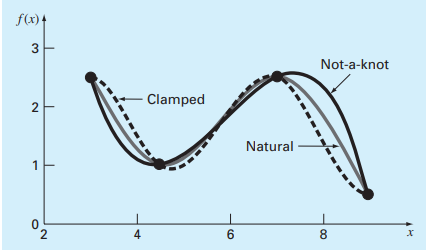
\includegraphics[scale=0.8]{fig_18_5}
   \caption{\textsf{Comparison of the clamped (with zero first derivatives), not-a-knot, and natural splines for the
   data from Table 18.1.}}\label{fig:fig_18_5}
\end{figure}

\section{PIECEWISE INTERPOLATION IN MATLAB}
MATLAB has several built-in functions to implement piecewise interpolation. The spline
function performs cubic spline interpolation as described in this chapter. The pchip function implements piecewise cubic Hermite interpolation. The interp1 function can also
implement spline and Hermite interpolation, but can also perform a number of other types
of piecewise interpolation.

\subsection{MATLAB Function: spline}
Cubic splines can be easily computed with the built-in MATLAB function, spline. It has
the general syntax,
\begin{lstlisting}[numbers=none]
    
    yy = spline(x, y, xx)
\end{lstlisting}

where x and y = vectors containing the values that are to be interpolated, and yy = a vector
containing the results of the spline interpolation as evaluated at the points in the vector xx.
By default, spline uses the not-a-knot condition. However, if y contains two more
values than x has entries, then the first and last value in y are used as the derivatives at the
end points. Consequently, this option provides the means to implement the clamped-end
condition.

\begin{exmp} \textbf{Splines in MATLAB}
    \noindent\textit{Problem Statement.} Runge’s function is a notorious example of a function that cannot
    be fit well with polynomials (recall Example 17.7):
    \begin{equation}
        f(x)=\frac{1}{1+25 x^{2}}\nonumber
    \end{equation}

Use MATLAB to fit nine equally spaced data points sampled from this function in the interval $[-1,1]$. Employ (a) a not-a-knot spline and (b) a clamped spline with end slopes of $f_{1}^{\prime}=1$ and $f_{n-1}^{\prime}=-4$.\\
\noindent \textbf{Solution.} (a) The nine equally spaced data points can be generated as in

\begin{lstlisting}[numbers=none]
>> x = linspace(-1,1,9);
>> y = 1./(1+25*x.^2);
\end{lstlisting}

Next, a more finely spaced vector of values can be generated so that we can create a smooth
plot of the results as generated with the spline function:

\begin{lstlisting}[numbers=none]
>> xx = linspace(-1,1);
>> yy = spline(x,y,xx);
\end{lstlisting}

Recall that linspace automatically creates 100 points if the desired number of points are
not specified. Finally, we can generate values for Runge's function itself and display them
along with the spline fit and the original data:

\begin{lstlisting}[numbers=none]
>> yr = 1./(1+25*xx.^2);
>> plot(x,y,'o',xx,yy,xx,yr,'--')
\end{lstlisting}
As in Fig. 18.6, the not-a-knot spline does a nice job of following Runge's function without exhibiting wild oscillations between the points.
\\(b) The clamped condition can be implemented by creating a new vector yc that has the
desired first derivatives as its first and last elements. The new vector can then be used to

\begin{figure}[H]
    \centering
    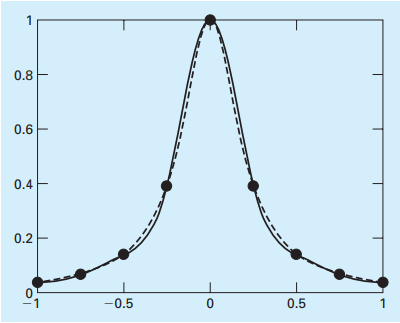
\includegraphics[scale=0.6]{fig_18_6}
   \caption{\textsf{Comparison of Runge's function (dashed line) with a 9-point not-a-knot spline fit generated with
   MATLAB (solid line).}}\label{fig:fig_18_6}
\end{figure}

\begin{figure}[H]
    \centering
    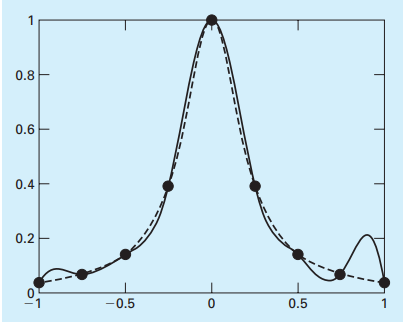
\includegraphics[scale=0.6]{fig_18_7}
   \caption{\textsf{Comparison of Runge's function (dashed line) with a 9-point clamped end spline fit generated
   with MATLAB (solid line). Note that first derivatives of 1 and -4 are specified at the left and
   right boundaries, respectively.}}\label{fig:fig_18_7}
\end{figure}
generate and plot the spline fit:

\begin{lstlisting}[numbers=none]
>> yc = [1 y -4];
>> yyc = spline(x,yc,xx);
>> plot(x,y,'o',xx,yyc,xx,yr,'--')
\end{lstlisting}
As in Fig. 18.7, the clamped spline now exhibits some oscillations because of the artificial
slopes that we have imposed at the boundaries. In other examples, where we have knowledge of the true first derivatives, the clamped spline tends to improve the fit.

\end{exmp}

\subsection{MATLAB Function: interp1}
The built-in function interp1 provides a handy means to implement a number of different types of piecewise one-dimensional interpolation. It has the general syntax

\begin{lstlisting}[numbers=none]
yi = interp1(x, y, xi, 'method')
\end{lstlisting}

where x and y = vectors containing values that are to be interpolated, yi = a vector containing the results of the interpolation as evaluated at the points in the vector xi, and
'method' = the desired method. The various methods are

\begin{itemize}
    \item 'nearest'—nearest neighbor interpolation. This method sets the value of an interpolated point to the value of the nearest existing data point. Thus, the interpolation
    looks like a series of plateaus, which can be thought of as zero-order polynomials.
    \item 'linear'—linear interpolation. This method uses straight lines to connect the points.
    \item 'spline'—piecewise cubic spline interpolation. This is identical to the spline
    function.
    \item 'pchip' and 'cubic'—piecewise cubic Hermite interpolation.
\end{itemize}

If the 'method' argument is omitted, the default is linear interpolation.
The pchip option (short for “piecewise cubic Hermite interpolation”) merits more
discussion. As with cubic splines, pchip uses cubic polynomials to connect data points
with continuous first derivatives. However, it differs from cubic splines in that the second
derivatives are not necessarily continuous. Further, the first derivatives at the knots will not
be the same as for cubic splines. Rather, they are expressly chosen so that the interpolation
is “shape preserving.” That is, the interpolated values do not tend to overshoot the data
points as can sometimes happen with cubic splines.
Therefore, there are trade-offs between the spline and the pchip options. The results
of using spline will generally appear smoother because the human eye can detect discontinuities in the second derivative. In addition, it will be more accurate if the data are values of a smooth function. On the other hand, pchip has no overshoots and less oscillation
if the data are not smooth. These trade-offs, as well as those involving the other options, are
explored in the following example.

\begin{exmp} \textbf{Trade-Offs Using interp1}
    \noindent\textit{Problem Statement.} You perform a test drive on an automobile where you alternately
    accelerate the automobile and then hold it at a steady velocity. Note that you never decelerate during the experiment. The time series of spot measurements of velocity can be
    tabulated as
$$
    \begin{array}{ccccccccccc}
        \hline \boldsymbol{t} & 0 & 20 & 40 & 56 & 68 & 80 & 84 & 96 & 104 & 110 \\
        \boldsymbol{v} & 0 & 20 & 20 & 38 & 80 & 80 & 100 & 100 & 125 & 125 \\
        \hline
        \end{array}
$$
Use MATLAB's interp1 function to fit these data with (a) linear interpolation, (b) nearest neighbor, (c) cubic spline with not-a-knot end conditions, and (d) piecewise cubic
Hermite interpolation.
    \noindent \textbf{Solution.} (a) The data can be entered, fit with linear interpolation, and plotted with the
    following commands:

    \begin{lstlisting}[numbers=none]
>> t = [0 20 40 56 68 80 84 96 104 110];
>> v = [0 20 20 38 80 80 100 100 125 125];
>> tt = linspace(0,110);
>> vl = interp1(t,v,tt);
>> plot(t,v,'o',tt,vl)
    \end{lstlisting}
    The results (Fig. 18.8a) are not smooth, but do not exhibit any overshoot.
    (b) The commands to implement and plot the nearest neighbor interpolation are
    \begin{lstlisting}[numbers=none]
>> vn = interp1(t,v,tt,'nearest');
>> plot(t,v,'o',tt,vn)
    \end{lstlisting}

    \begin{figure}[H]
        \centering
        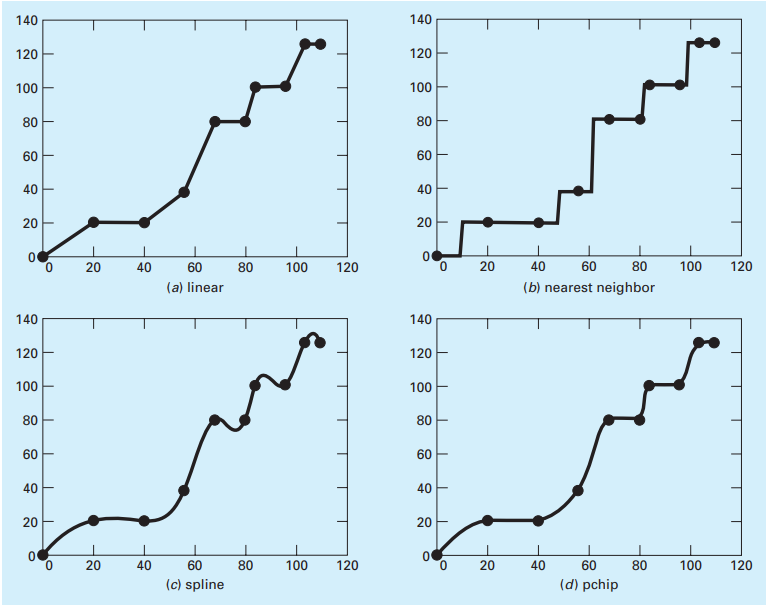
\includegraphics[scale=0.6]{fig_18_8}
       \caption{\textsf{Use of several options of the interp1 function to perform piecewise polynomial interpolation on a velocity time series
       for an automobile.}}\label{fig:fig_18_8}
    \end{figure}

    As in Fig. 18.8b, the results look like a series of plateaus. This option is neither a smooth
nor an accurate depiction of the underlying process.
(c) The commands to implement the cubic spline are

\begin{lstlisting}[numbers=none]
>> vs = interp1(t,v,tt,'spline');
>> plot(t,v,'o',tt,vs)
\end{lstlisting}

These results (Fig. 18.8c) are quite smooth. However, severe overshoot occurs at several
locations. This makes it appear that the automobile decelerated several times during the
experiment.

(d) The commands to implement the piecewise cubic Hermite interpolation are

\begin{lstlisting}[numbers=none]
>> vh = interp1(t,v,tt,'pchip');
>> plot(t,v,'o',tt,vh)
\end{lstlisting}

For this case, the results (Fig. 18.8d) are physically realistic. Because of its shape-preserving
nature, the velocities increase monotonically and never exhibit deceleration. Although the
result is not as smooth as for the cubic splines, continuity of the first derivatives at the knots
makes the transitions between points more gradual and hence more realistic.

\end{exmp}

\section{MULTIDIMENSIONAL INTERPOLATION}
The interpolation methods for one-dimensional problems can be extended to multidimensional interpolation. In this section, we will describe the simplest case of two-dimensional
interpolation in Cartesian coordinates. In addition, we will describe MATLAB's capabilities for multidimensional interpolation.

\subsection{Bilinear Interpolation}

Two-dimensional interpolation deals with determining intermediate values for functions
of two variables z = f ($x\textsubscript{i}$, $y\textsubscript{i}$). As depicted in Fig. 18.9, we have values at four points:
f ($x\textsubscript{1}$, $y\textsubscript{1}$), f ($x\textsubscript{2}$, y1), f ($x\textsubscript{1}$, $y\textsubscript{2}$), and f ($x\textsubscript{2}$, $y\textsubscript{2}$). We want to interpolate between these points

\begin{figure}[H]
    \centering
    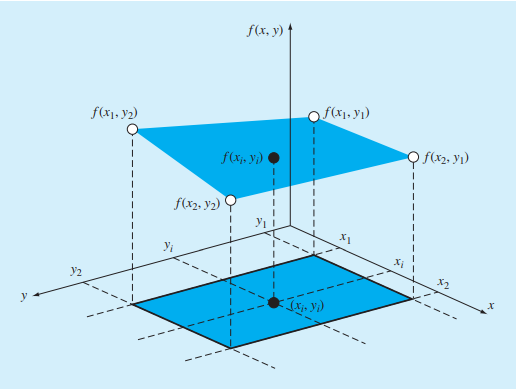
\includegraphics[scale=0.6]{fig_18_9}
   \caption{\textsf{Graphical depiction of two-dimensional bilinear interpolation where an intermediate value (filled
   circle) is estimated based on four given values (open circles).}}\label{fig:fig_18_9}
\end{figure}

\begin{figure}[H]
    \centering
    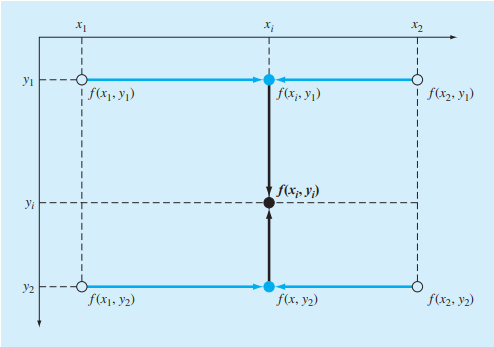
\includegraphics[scale=0.6]{fig_18_10}
   \caption{\textsf{Two-dimensional bilinear interpolation can be implemented by first applying one-dimensional
   linear interpolation along the x dimension to determine values at $x\textsubscript{i}$
   . These values can then be
   used to linearly interpolate along the y dimension to yield the final result at $x\textsubscript{i}$
   , $y\textsubscript{i}$
   ...}}\label{fig:fig_18_10}
\end{figure}

to estimate the value at an intermediate point f ($x\textsubscript{i}$, $y\textsubscript{i}$). If we use a linear function, the result is a plane connecting the points as in Fig. 18.9. Such functions are called bilinear.
A simple approach for developing the bilinear function is depicted in Fig. 18.10. First,
we can hold the y value fixed and apply one-dimensional linear interpolation in the x direction. Using the Lagrange form, the result at ($x\textsubscript{i}$, $y\textsubscript{i}$) is

\begin{equation}
    \tag{18.29}
f\left(x_{i}, y_{1}\right)=\frac{x_{i}-x_{2}}{x_{1}-x_{2}} f\left(x_{1}, y_{1}\right)+\frac{x_{i}-x_{1}}{x_{2}-x_{1}} f\left(x_{2}, y_{1}\right)
\end{equation}
and at $\left(x_{i}, y_{2}\right)$ is
\begin{equation}
    \tag{18.30}
f\left(x_{i}, y_{2}\right)=\frac{x_{i}-x_{2}}{x_{1}-x_{2}} f\left(x_{1}, y_{2}\right)+\frac{x_{i}-x_{1}}{x_{2}-x_{1}} f\left(x_{2}, y_{2}\right)
\end{equation}
These points can then be used to linearly interpolate along the $y$ dimension to yield the final result:
\begin{equation}
    \tag{18.31}
f\left(x_{i}, y_{i}\right)=\frac{y_{i}-y_{2}}{y_{1}-y_{2}} f\left(x_{i}, y_{1}\right)+\frac{y_{i}-y_{1}}{y_{2}-y_{1}} f\left(x_{i}, y_{2}\right)
\end{equation}
A single equation can be developed by substituting Eqs. (18.29) and (18.30) into Eq. (18.31) to give
\begin{equation}
    \tag{18.32}
\begin{aligned}
f\left(x_{i}, y_{i}\right)=& \frac{x_{i}-x_{2}}{x_{1}-x_{2}} \frac{y_{i}-y_{2}}{y_{1}-y_{2}} f\left(x_{1}, y_{1}\right)+\frac{x_{i}-x_{1}}{x_{2}-x_{1}} \frac{y_{i}-y_{2}}{y_{1}-y_{2}} f\left(x_{2}, y_{1}\right) \\
&+\frac{x_{i}-x_{2}}{x_{1}-x_{2}} \frac{y_{i}-y_{1}}{y_{2}-y_{1}} f\left(x_{1}, y_{2}\right)+\frac{x_{i}-x_{1}}{x_{2}-x_{1}} \frac{y_{i}-y_{1}}{y_{2}-y_{1}} f\left(x_{2}, y_{2}\right)
\end{aligned}
\end{equation}

\begin{exmp} \textbf{Bilinear Interpolation}
    \noindent\textit{Problem Statement.}Suppose you have measured temperatures at a number of coordinates on the surface of a rectangular heated plate:

    \begin{equation}
    \begin{array}{ll}
    T(2,1)=60 & T(9,1)=57.5 \\
    T(2,6)=55 & T(9,6)=70
    \end{array}\nonumber
\end{equation}
    Use bilinear interpolation to estimate the temperature at $x_{i}=5.25$ and $y_{i}=4.8$.
    \noindent \textbf{Solution.} Substituting these values into Eq. (18.32) gives
    \begin{equation}
    \begin{aligned}
    f(5.25,4.8)=& \frac{5.25-9}{2-9} \frac{4.8-6}{1-6} 60+\frac{5.25-2}{9-2} \frac{4.8-6}{1-6} 57.5 \\
    &+\frac{5.25-9}{2-9} \frac{4.8-1}{6-1} 55+\frac{5.25-2}{9-2} \frac{4.8-1}{6-1} 70=61.2143
    \end{aligned}\nonumber
\end{equation}

\end{exmp}

\subsection{ Multidimensional Interpolation in MATLAB}
MATLAB has two built-in functions for two- and three-dimensional piecewise interpolation: interp2 and interp3. As you might expect from their names, these functions operate in a similar fashion to interp1 (Section 18.5.2). For example, a simple representation
of the syntax of interp2 is 
\begin{lstlisting}[numbers=none]
zi = interp2(x, y, z, xi, yi, 'method')
\end{lstlisting}
where x and y = matrices containing the coordinates of the points at which the values in
the matrix z are given, zi = a matrix containing the results of the interpolation as evaluated at the points in the matrices xi and yi, and method = the desired method. Note that
the methods are identical to those used by interp1; that is, linear, nearest, spline,
and cubic.\\
As with interp1, if the method argument is omitted, the default is linear interpolation.
For example, interp2 can be used to make the same evaluation as in Example 18.6 as

\begin{lstlisting}[numbers=none]
>> x=[2 9];
>> y=[1 6];
>> z=[60 57.5;55 70];
>> interp2(x,y,z,5.25,4.8)
ans =
61.2143
\end{lstlisting}

\section{CASE STUDY: HEAT TRANSFER}

\noindent \textbf{Background.}
Lakes in the temperate zone can become thermally stratified during the summer. As depicted in Fig. 18.11, warm, buoyant water near the surface overlies colder, denser bottom water. Such stratification effectively divides the lake vertically into two layers: the epilimnion and the hypolimnion, separated by a plane called the thermocline.

Thermal stratification has great significance for environmental engineers and scientists studying such systems. In particular, the thermocline greatly diminishes mixing between the two layers. As a result, decomposition of organic matter can lead to severe depletion of oxygen in the isolated bottom waters.

The location of the thermocline can be defined as the inflection point of the temperaturedepth curve-that is, the point at which $d^{2} T / d z^{2}=0$. It is also the point at which the absolute value of the first derivative or gradient is a maximum.

The temperature gradient is important in its own right because it can be used in conjunction with Fourier's law to determine the heat flux across the thermocline:
\begin{equation}
    \tag{18.33}
J=-D \rho C \frac{d T}{d z}
\end{equation}
where $J=$ heat flux $\left[\mathrm{cal} /\left(\mathrm{cm}^{2} \cdot \mathrm{s}\right)\right], \alpha=$ an eddy diffusion coefficient $\left(\mathrm{cm}^{2} / \mathrm{s}\right), \rho=$ density $\left(\cong 1 \mathrm{~g} / \mathrm{cm}^{3}\right)$, and $C=$ specific heat $[\cong 1 \mathrm{cal} /(\mathrm{g} \cdot \mathrm{C})]$.

In this case study, natural cubic splines are employed to determine the thermocline depth and temperature gradient for Platte Lake, Michigan (Table 18.3). The latter is also used to determine the heat flux for the case where $\alpha=0.01 \mathrm{~cm}^{2} / \mathrm{s}$.

\begin{figure}[H]
    \centering
    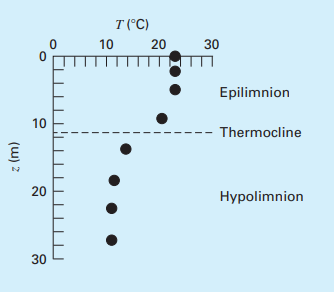
\includegraphics[scale=0.6]{fig_18_11}
   \caption{\textsf{Temperature versus depth during summer for Platte Lake, Michigan.
   }}\label{fig:fig_18_11}
\end{figure}

\noindent \textbf{Solution.}
As just described, we want to use natural spline end conditions to perform this
analysis. Unfortunately, because it uses not-a-knot end conditions, the built-in MATLAB
spline function does not meet our needs. Further, the spline function does not return the
first and second derivatives we require for our analysis.
However, it is not difficult to develop our own M-file to implement a natural spline
and return the derivatives. Such a code is shown in Fig. 18.12. After some preliminary error
trapping, we set up and solve Eq. (18.27) for the second-order coefficients (c). Notice how

\begin{figure}[H]
    \centering
    
\includegraphics[scale=0.6]{fig_18_12}
   \caption{\textsf{M-file to determine intermediate values and derivatives with a natural spline. Note that the diff
   function employed for error trapping is described in Section 21.7.1.}}\label{fig:fig_18_12}
\end{figure}
\begin{lstlisting}[numbers=none]
function [yy,dy,d2] = natspline(x,y,xx)
% natspline: natural spline with differentiation
% [yy,dy,d2] = natspline(x,y,xx): uses a natural cubic spline
% interpolation to find yy, the values of the underlying function
% y at the points in the vector xx. The vector x specifies the
% points at which the data y is given.
% input:
% x = vector of independent variables
% y = vector of dependent variables
% xx = vector of desired values of dependent variables
% output:
% yy = interpolated values at xx
% dy = first derivatives at xx
% d2 = second derivatives at xx
n = length(x);
if length(y)~=n, error('x and y must be same length'); end
if any(diff(x)<=0),error('x not strictly ascending'),end
m = length(xx);
b = zeros(n,n);
aa(1,1) = 1; aa(n,n) = 1; %set up Eq. 18.27
bb(1)=0; bb(n)=0;
for i = 2:n-1
aa(i,i-1) = h(x, i - 1);
aa(i,i) = 2 * (h(x, i - 1) + h(x, i));
aa(i,i+1) = h(x, i);
bb(i) = 3 * (fd(i + 1, i, x, y) - fd(i, i - 1, x, y));
end
c=aa\bb'; %solve for c coefficients
for i = 1:n - 1 %solve for a, b and d coefficients
a(i) = y(i);
b(i) = fd(i + 1, i, x, y) - h(x, i) / 3 * (2 * c(i) + c(i + 1));
d(i) = (c(i + 1) - c(i)) / 3 / h(x, i);
end
for i = 1:m %perform interpolations at desired values
[yy(i),dy(i),d2(i)] = SplineInterp(x, n, a, b, c, d, xx(i));
end
end
function hh = h(x, i)
hh = x(i + 1) - x(i);
end
function fdd = fd(i, j, x, y)
fdd = (y(i) - y(j)) / (x(i) - x(j));
end
function [yyy,dyy,d2y]=SplineInterp(x, n, a, b, c, d, xi)
for ii = 1:n - 1
if xi >= x(ii) - 0.000001 & xi <= x(ii + 1) + 0.000001
yyy=a(ii)+b(ii)*(xi-x(ii))+c(ii)*(xi-x(ii))^2+d(ii)...
*(xi-x(ii))^3;
dyy=b(ii)+2*c(ii)*(xi-x(ii))+3*d(ii)*(xi-x(ii))^2;
d2y=2*c(ii)+6*d(ii)*(xi-x(ii));
break
end
end
end
\end{lstlisting}

we use two subfunctions, h and fd, to compute the required finite differences. Once
Eq. (18.27) is set up, we solve for the c's with back division. A loop is then employed to
generate the other coefficients (a, b, and d).
At this point, we have all we need to generate intermediate values with the cubic
equation:
$$
f(x)=a_{i}+b_{i}\left(x-x_{i}\right)+c_{i}\left(x-x_{i}\right)^{2}+d_{i}\left(x-x_{i}\right)^{3}
$$
We can also determine the first and second derivatives by differentiating this equation twice to give
$$
\begin{aligned}
&f^{\prime}(x)=b_{i}+2 c_{i}\left(x-x_{i}\right)+3 d_{i}\left(x-x_{i}\right)^{2} \\
&f^{\prime \prime}(x)=2 c_{i}+6 d_{i}\left(x-x_{i}\right)
\end{aligned}
$$
As in Fig. 18.12, these equations can then be implemented in another subfunction,
SplineInterp, to determine the values and the derivatives at the desired intermediate
values.
Here is a script file that uses the natspline function to generate the spline and create
plots of the results: 

\begin{lstlisting}[numbers=none]
    [TT,dT,dT2] = natspline(z,T,zz);
    subplot(1,3,1),plot(T,z,'o',TT,zz)
    title('(a) T'),legend('data','T')
    set(gca,'YDir','reverse'),grid
    subplot(1,3,2),plot(dT,zz)
    title('(b) dT/dz')
    set(gca,'YDir','reverse'),grid
    subplot(1,3,3),plot(dT2,zz)
    title('(c) d2T/dz2')
    set(gca,'YDir','reverse'),grid
\end{lstlisting}

As in Fig. 18.13, the thermocline appears to be located at a depth of about 11.5 m. We
can use root location (zero second derivative) or optimization methods (minimum first
derivative) to refine this estimate. The result is that the thermocline is located at 11.35 m
where the gradient is -1.61 °C/m.

\begin{figure}[H]
    \centering
    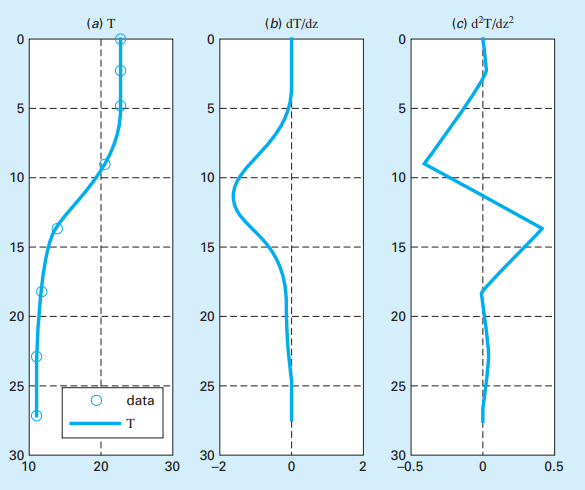
\includegraphics[scale=0.6]{fig_18_13}
   \caption{\textsf{Plots of (a) temperature, (b) gradient, and (c) second derivative versus depth (m) generated with
   the cubic spline program. The thermocline is located at the inflection point of the temperaturedepth curve.}}\label{fig:fig_18_13}
\end{figure}

The gradient can be used to compute the heat flux across the thermocline with
Eq. (18.33):
\begin{equation}
    \nonumber
    J=-0.01 \frac{\mathrm{cm}^{2}}{\mathrm{~s}} \times 1 \frac{\mathrm{g}}{\mathrm{cm}^{3}} \times 1 \frac{\mathrm{cal}}{\mathrm{g} \cdot{ }^{\circ} \mathrm{C}} \times\left(-1.61 \frac{{ }^{\circ} \mathrm{C}}{\mathrm{m}}\right) \times \frac{1 \mathrm{~m}}{100 \mathrm{~cm}} \times \frac{86,400 \mathrm{~s}}{\mathrm{~d}}=13.9 \frac{\mathrm{cal}}{\mathrm{cm}^{2} \cdot \mathrm{d}}
    \end{equation}

    The foregoing analysis demonstrates how spline interpolation can be used for engineering and scientific problem solving. However, it also is an example of numerical differentiation. As such, it illustrates how numerical approaches from different areas can be used
    in tandem for problem solving. We will be describing the topic of numerical differentiation
    in detail in Chap. 21.

    \vspace{5mm}

    \section{PROBLEMS}
    \begin{multicols}{2}
    \noindent\textit{18.1 Given the data}\vspace{5mm}

    \begin{tabular}{lcccccc}
    \hline $\boldsymbol{x}$ & 1 & 2 & $2.5$ & 3 & 4 & 5 \\
    $\boldsymbol{f}(\boldsymbol{x})$ & 1 & 5 & 7 & 8 & 2 & 1 \\
    \hline
    \end{tabular}\\
    Fit these data with (a) a cubic spline with natural end conditions, (b) a cubic spline with not-a-knot end conditions, and (c) piecewise cubic Hermite interpolation.\\
    \noindent\textit{18.2 A reactor is thermally stratified as in the following table:}\vspace{2mm}\\
    \begin{tabular}{lccccccc}
    \hline Depth, m & 0 & $0.5$ & 1 & $1.5$ & 2 & $2.5$ & 3 \\
    Temperature, ${ }^{\circ} \mathbf{C}$ & 70 & 70 & 55 & 22 & 13 & 10 & 10 \\
    \hline
    \end{tabular}\\
    Based on these temperatures, the tank can be idealized as two zones separated by a strong temperature gradient or thermocline. The depth of the thermocline can be defined as the inflection point of the temperature-depth curve-that is, the point at which $d^{2} T / d z^{2}=0$. At this depth, the heat flux from the surface to the bottom layer can be computed with Fourier's law:
    $$
    J=-k \frac{d T}{d z}
    $$
Use a clamped cubic spline fit with zero end derivatives to determine the thermocline depth. If $k=0.01 \mathrm{cal} /\left(\mathrm{s} \cdot \mathrm{cm} \cdot{ }^{\circ} \mathrm{C}\right)$ compute the flux across this interface.
    
\noindent\textit{18.3 The following is the built-in humps function that MATLAB uses to demonstrate some of its numerical capabilities:}\vspace{5mm}
    $$
    f(x)=\frac{1}{(x-0.3)^{2}+0.01}+\frac{1}{(x-0.9)^{2}+0.04}-6
    $$
    The humps function exhibits both flat and steep regions over a relatively short $x$ range. Here are some values that have been generated at intervals of $0.1$ over the range from $x=0$ to 1 :\\
$$
        \begin{array}{lcccccc}
            \hline \boldsymbol{x} & 0 & 0.1 & 0.2 & 0.3 & 0.4 & 0.5 \\
            \boldsymbol{f}(\boldsymbol{x}) & 5.176 & 15.471 & 45.887 & 96.500 & 47.448 & 19.000 \\
            \boldsymbol{x} & 0.6 & 0.7 & 0.8 & 0.9 & 1 & \\
            \boldsymbol{f ( x )} & 11.692 & 12.382 & 17.846 & 21.703 & 16.000 & \\
            \hline
        \end{array}
$$
    Fit these data with a (a) cubic spline with not-a-knot end conditions and (b) piecewise cubic Hermite interpolation. In both cases, create a plot comparing the fit with the exact humps function.
    
    \noindent\textit{18.4 Develop a plot of a cubic spline fit of the following data with (a) natural end conditions and (b) not-a-knot end conditions. In addition, develop a plot using (c) piecewise
    cubic Hermite interpolation.}\vspace{5mm}

        $$
        \begin{array}{lcccccc}
            \hline \boldsymbol{x} & 0 & 100 & 200 & 400 \\
            \boldsymbol{f}(\boldsymbol{x}) & 0 & $0.82436$ & $1.00000$ & $0.73576$ \\
            \boldsymbol{x} & 600 & 800 & 1000 & \\
            \boldsymbol{f}(\boldsymbol{x}) & $0.40601$ & $0.19915$ & $0.09158$ & \\
            \hline
        \end{array}
        $$
        In each case, compare your plot with the following equation which was used to generate the data:
        $$
        f(x)=\frac{x}{200} e^{-x / 200+1}
        $$
        
        \noindent\textit{18.5 The following data are sampled from the step function depicted in Fig. 18.1:}
        $$
        \begin{array}{lcccccc}
            \hline \boldsymbol{x} & -1 & -0.6 & -0.2 & 0.2 & 0.6 & 1 \\
            \boldsymbol{f}(\boldsymbol{x}) & 0 & 0 & 0 & 1 & 1 & 1 \\
            \hline
        \end{array}
        $$
        Fit these data with a (a) cubic spline with not-a-knot end conditions, (b) cubic spline with zero-slope clamped end conditions, and (c) piecewise cubic Hermite interpolation. In each case, create a plot comparing the fit with the step function. 
        \noindent\textit{18.6 Develop an M-file to compute a cubic spline fit with natural end conditions. Test your code by using it to duplicate Example 18.3.}
        \noindent\textit{18.7 The following data were generated with the fifthorder polynomial: $f(x)=0.0185 x^{5}-0.444 x^{4}+3.9125 x^{3}-$ $15.456 x^{2}+27.069 x-14.1:$
        (a) Fit these data with a cubic spline with not-a-knot end conditions. Create a plot comparing the fit with the function. (b) Repeat (a) but use clamped end conditions where the end slopes are set at the exact values as determined by differentiating the function.}
        \noindent\textit{18.8 Bessel functions often arise in advanced engineering and scientific analyses such as the study of electric fields. These functions are usually not amenable to straightforward evaluation and, therefore, are often compiled in standard mathematical tables. For example,}
        
$$
        \begin{array}{lcccccc}
            \hline \boldsymbol{x} & 1.8 & 2 & 2.2 & 2.4 & 2.6 \\
            \boldsymbol{J}_{\mathbf{1}}(\boldsymbol{x}) & 0.5815 & 0.5767 & 0.556 & 0.5202 & 0.4708 \\
            \hline
        \end{array}
$$
Estimate J1(2.1), (a) using an interpolating polynomial and
(b) using cubic splines. Note that the true value is 0.5683.
\noindent\textit{18.9 The following data define the sea-level concentration of dissolved oxygen for fresh water as a function of
temperature:}
$$
\begin{array}{lcccccc}
    \hline \boldsymbol{T}_{,}{ }^{\circ} \mathbf{C} & 0 & 8 & 16 & 24 & 32 & 40 \\
    \boldsymbol{o}, \mathbf{m g} / \mathbf{L} & 14.021 & 11.843 & 9.870 & 8.418 & 7.305 & 6.413 \\
    \hline
    \end{array}
$$
    Use MATLAB to fit the data with (a) piecewise linear interpolation, (b) a fifth-order polynomial, and (c) a spline. Display the results graphically and use each approach to estimate
    o(27). Note that the exact result is 7.986 mg/L
\noindent\textit{18.10 (a) Use MATLAB to fit a cubic spline to the following data to determine y at x = 1.5:}
$$
\begin{array}{lcccccc}
    \hline \boldsymbol{x} \mathbf{C} & 0 & 2 & 4 & 7 & 10 & 12 \\
    \boldsymbol{y} & 20 & 20 & 12 & 7 & 6 & 6 \\
    \hline
    \end{array}
$$
(b) Repeat (a), but with zero first derivatives at the end
knots.\\
\noindent\textit{18.11 Runge's function is written as
}
$$
f(x)=\frac{1}{1+25 x^{2}}
$$
Generate five equidistantly spaced values of this function over the interval: $[-1,1]$. Fit these data with (a) a fourthorder polynomial, (b) a linear spline, and (c) a cubic spline. Present your results graphically.
\noindent\textit{18.12 Use MATLAB to generate eight points from the function}

$$
f(t)=\sin ^{2} t
$$
from $t=0$ to $2 \pi$. Fit these data using (a) cubic spline with not-a-knot end conditions, (b) cubic spline with derivative end conditions equal to the exact values calculated with differentiation, and (c) piecewise cubic hermite interpolation. Develop plots of each fit as well as plots of the absolute error ( $E_{t}=$ approximation $-$ true) for each.\\
from t = 0 to 2$\pi$. Fit these data using (a) cubic spline with
not-a-knot end conditions, (b) cubic spline with derivative
end conditions equal to the exact values calculated with differentiation, and (c) piecewise cubic hermite interpolation.
Develop plots of each fit as well as plots of the absolute error
($E\textsubscript{t}$ = approximation - true) for each.

\noindent\textit{18.13 The drag coefficient for spheres such as sporting balls
is known to vary as a function of the Reynolds number Re, a
dimensionless number that gives a measure of the ratio of
inertial forces to viscous forces:}
$$
\operatorname{Re}=\frac{\rho V D}{\mu}
$$
where $\rho=$ the fluid's density $\left(\mathrm{kg} / \mathrm{m}^{3}\right), V=$ its velocity $(\mathrm{m} / \mathrm{s})$, $D=$ diameter $(\mathrm{m})$, and $\mu=$ dynamic viscosity $\left(\mathrm{N} \cdot \mathrm{s} / \mathrm{m}^{2}\right)$.
Although the relationship of drag to the Reynolds number is
sometimes available in equation form, it is frequently tabulated. For example, the following table provides values for a
smooth spherical ball:
$$
\begin{array}{lccccccc}
    \hline \operatorname{Re}\left(\times 10^{-4}\right) & 2 & 5.8 & 16.8 & 27.2 & 29.9 & 33.9 & \\
    \boldsymbol{C}_{D} & 0.52 & 0.52 & 0.52 & 0.5 & 0.49 & 0.44 & \\
    \operatorname{Re}\left(\times 10^{-4}\right) & 36.3 & 40 & 46 & 60 & 100 & 200 & 400 \\
    \boldsymbol{C}_{D} & 0.18 & 0.074 & 0.067 & 0.08 & 0.12 & 0.16 & 0.19 \\
    \hline
    \end{array}
$$
    (a) Develop a MATLAB function that employs the spline
    function to return a value of $C\textsubscript{D}$ as a function of
    the Reynolds number. The first line of the function
    should be
    \begin{lstlisting}[numbers=none]
        function CDout = Drag(ReCD,ReIn)
    \end{lstlisting}
    where ReCD = a 2-row matrix containing the table, ReIn =
    the Reynolds number at which you want to estimate the
    drag, and CDout = the corresponding drag coefficient.

    (b) Write a script that uses the function developed in part
    (a) to generate a labeled plot of the drag force versus velocity (recall Sec. 1.4). Use the following parameter values for the script: $D=22 \mathrm{~cm}, \rho=1.3 \mathrm{~kg} / \mathrm{m}^{3}$, and $\mu=1.78 \times 10^{-5} \mathrm{~Pa} \cdot \mathrm{s}$. Employ a range of velocities from 4 to $40 \mathrm{~m} / \mathrm{s}$ for your plot.
    18.14 The following function describes the temperature distribution on a rectangular plate for the range $-2 \leq x \leq 0$ and $0 \leq y \leq 3$
    $$
    T=2+x-y+2 x^{2}+2 x y+y^{2}
    $$
    Develop a script to: (a) Generate a meshplot of this function
    using the MATLAB function surfc. Employ the linspace
    function with default spacing (i.e., 100 interior points) to
    generate the x and y values. (b) Use the MATLAB function
    interp2 with the default interpolation option ('linear')
    to compute the temperature at x = -1.63 and y = 1.627.
    Determine the percent relative error of your result. (c) Repeat (b), but with 'spline'. Note: for parts (b) and (c), employ the linspace function with 9 interior points.

\end{multicols}


\end{document}

